% Written by make_deck_figures.py: edit the script, not this file.
% Correlation gamma on a made-up ranking: four skips, so the 13th ticker taken is at rank 17.
\documentclass[tikz,border=2pt]{standalone}
% Shared style for the L15a schematics, copied from L14a (November 19, 2026), \input by each Fig-L15a-*.tex.
% Copied from week-13/L13a/figs/jumphmm-diagram.tex (the week-12 schematic style): same fonts,
% ink, accent colors, boxes, and arrows, plus a monospace font for tool names and order
% statuses. The notebook SVG carries a dark palette added by theme_svg.py; every color here
% must be mapped there.
\usepackage[no-math]{fontspec}
\IfFontExistsTF{Arial}{\setsansfont{Arial}}{\setsansfont{TeX Gyre Heros}}
\renewcommand{\familydefault}{\sfdefault}
\IfFontExistsTF{Menlo}{\setmonofont[Scale=0.92]{Menlo}}{}
\usepackage{amsmath,amssymb}
\usetikzlibrary{arrows.meta,calc,positioning,decorations.pathreplacing}

\definecolor{vnink}{HTML}{202124}
\definecolor{gdblue}{HTML}{0091FF}
\definecolor{gdred}{HTML}{E02020}
\definecolor{gdgray}{HTML}{6D7278}
\definecolor{saorange}{HTML}{F08C00}
\definecolor{boxfill}{HTML}{F1F3F4}
\definecolor{orangefill}{HTML}{FFE8C7}
\definecolor{bluefill}{HTML}{E5F3FF}
\definecolor{redfill}{HTML}{FDE8E8}
\definecolor{gridgray}{HTML}{E3E5E8}

\tikzset{
  every picture/.append style={x=1cm, y=1cm, font=\sffamily\small, text=vnink},
  % boxes and arrows, as in the L12a schematics
  flow/.style={draw=vnink, line width=0.9pt, -{Latex[length=2.4mm, width=1.7mm]}},
  feedback/.style={draw=saorange, line width=1.2pt, -{Latex[length=2.6mm, width=1.9mm]}, rounded corners=6pt},
  sumbox/.style={draw=vnink, fill=boxfill, line width=0.8pt, rounded corners=3pt, inner sep=5pt, align=center},
  note/.style={text=gdgray, font=\sffamily\footnotesize, align=center},
  state/.style={circle, draw=vnink, fill=white, line width=1.0pt, minimum size=1.1cm, inner sep=0pt, font=\sffamily\normalsize},
  % plots, as in the L10b profit diagrams
  axis/.style={draw=vnink, line width=0.8pt, -{Latex[length=2.6mm, width=1.8mm]}},
  spine/.style={draw=vnink, line width=0.8pt},
  curve/.style={draw=vnink, line width=1.6pt, line join=round, line cap=round},
  series/.style={draw=gdgray, line width=0.9pt, line join=round},
  drop/.style={draw=gdgray, line width=0.8pt, dash pattern=on 3pt off 2pt},
  pt/.style={circle, draw=vnink, fill=white, line width=1.0pt, inner sep=0pt, minimum size=2.0mm},
}


\begin{document}
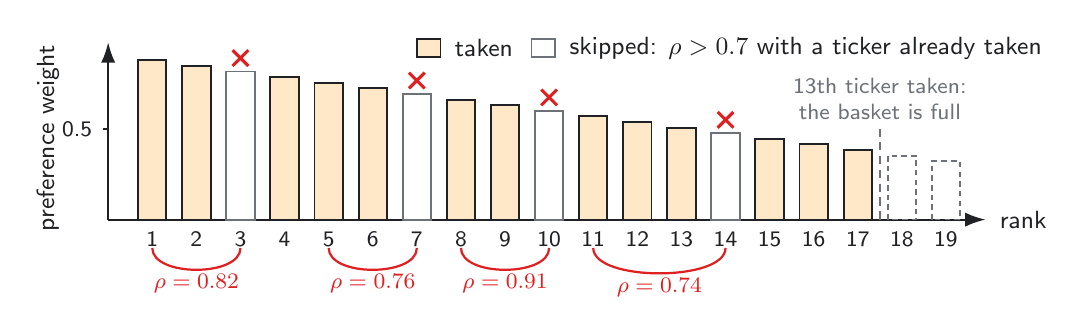
\begin{tikzpicture}
  \draw[axis] (0, 0) -- (11.144, 0);
  \draw[axis] (0, 0) -- (0, 2.254);
  \draw[spine] (0, 1.15) -- (-0.07, 1.15);
  \node[anchor=east, font=\sffamily\footnotesize] at (-0.08, 1.15) {0.5};
  \node[font=\sffamily\small, rotate=90, anchor=south] at (-0.5, 1.035) {preference weight};
  \node[font=\sffamily\small, anchor=west] at (11.2, 0) {rank};
  \node[font=\sffamily\footnotesize, anchor=north] at (0.56, -0.03) {1};
  \filldraw[fill=orangefill, draw=vnink, line width=0.7pt] (0.38, 0) rectangle (0.74, 2.024);
  \node[font=\sffamily\footnotesize, anchor=north] at (1.12, -0.03) {2};
  \filldraw[fill=orangefill, draw=vnink, line width=0.7pt] (0.94, 0) rectangle (1.3, 1.9527);
  \node[font=\sffamily\footnotesize, anchor=north] at (1.68, -0.03) {3};
  \filldraw[fill=white, draw=gdgray, line width=0.7pt] (1.5, 0) rectangle (1.86, 1.8814);
  \draw[draw=gdred, line width=1.1pt] (1.58, 1.9514) -- (1.78, 2.1514) (1.58, 2.1514) -- (1.78, 1.9514);
  \node[font=\sffamily\footnotesize, anchor=north] at (2.24, -0.03) {4};
  \filldraw[fill=orangefill, draw=vnink, line width=0.7pt] (2.06, 0) rectangle (2.42, 1.8101);
  \node[font=\sffamily\footnotesize, anchor=north] at (2.8, -0.03) {5};
  \filldraw[fill=orangefill, draw=vnink, line width=0.7pt] (2.62, 0) rectangle (2.98, 1.7388);
  \node[font=\sffamily\footnotesize, anchor=north] at (3.36, -0.03) {6};
  \filldraw[fill=orangefill, draw=vnink, line width=0.7pt] (3.18, 0) rectangle (3.54, 1.6675);
  \node[font=\sffamily\footnotesize, anchor=north] at (3.92, -0.03) {7};
  \filldraw[fill=white, draw=gdgray, line width=0.7pt] (3.74, 0) rectangle (4.1, 1.5962);
  \draw[draw=gdred, line width=1.1pt] (3.82, 1.6662) -- (4.02, 1.8662) (3.82, 1.8662) -- (4.02, 1.6662);
  \node[font=\sffamily\footnotesize, anchor=north] at (4.48, -0.03) {8};
  \filldraw[fill=orangefill, draw=vnink, line width=0.7pt] (4.3, 0) rectangle (4.66, 1.5249);
  \node[font=\sffamily\footnotesize, anchor=north] at (5.04, -0.03) {9};
  \filldraw[fill=orangefill, draw=vnink, line width=0.7pt] (4.86, 0) rectangle (5.22, 1.4536);
  \node[font=\sffamily\footnotesize, anchor=north] at (5.6, -0.03) {10};
  \filldraw[fill=white, draw=gdgray, line width=0.7pt] (5.42, 0) rectangle (5.78, 1.3823);
  \draw[draw=gdred, line width=1.1pt] (5.5, 1.4523) -- (5.7, 1.6523) (5.5, 1.6523) -- (5.7, 1.4523);
  \node[font=\sffamily\footnotesize, anchor=north] at (6.16, -0.03) {11};
  \filldraw[fill=orangefill, draw=vnink, line width=0.7pt] (5.98, 0) rectangle (6.34, 1.311);
  \node[font=\sffamily\footnotesize, anchor=north] at (6.72, -0.03) {12};
  \filldraw[fill=orangefill, draw=vnink, line width=0.7pt] (6.54, 0) rectangle (6.9, 1.2397);
  \node[font=\sffamily\footnotesize, anchor=north] at (7.28, -0.03) {13};
  \filldraw[fill=orangefill, draw=vnink, line width=0.7pt] (7.1, 0) rectangle (7.46, 1.1684);
  \node[font=\sffamily\footnotesize, anchor=north] at (7.84, -0.03) {14};
  \filldraw[fill=white, draw=gdgray, line width=0.7pt] (7.66, 0) rectangle (8.02, 1.0971);
  \draw[draw=gdred, line width=1.1pt] (7.74, 1.1671) -- (7.94, 1.3671) (7.74, 1.3671) -- (7.94, 1.1671);
  \node[font=\sffamily\footnotesize, anchor=north] at (8.4, -0.03) {15};
  \filldraw[fill=orangefill, draw=vnink, line width=0.7pt] (8.22, 0) rectangle (8.58, 1.0258);
  \node[font=\sffamily\footnotesize, anchor=north] at (8.96, -0.03) {16};
  \filldraw[fill=orangefill, draw=vnink, line width=0.7pt] (8.78, 0) rectangle (9.14, 0.9545);
  \node[font=\sffamily\footnotesize, anchor=north] at (9.52, -0.03) {17};
  \filldraw[fill=orangefill, draw=vnink, line width=0.7pt] (9.34, 0) rectangle (9.7, 0.8832);
  \node[font=\sffamily\footnotesize, anchor=north] at (10.08, -0.03) {18};
  \draw[draw=gdgray, line width=0.6pt, dash pattern=on 2pt off 1.5pt] (9.9, 0) rectangle (10.26, 0.8119);
  \node[font=\sffamily\footnotesize, anchor=north] at (10.64, -0.03) {19};
  \draw[draw=gdgray, line width=0.6pt, dash pattern=on 2pt off 1.5pt] (10.46, 0) rectangle (10.82, 0.7406);
  \draw[draw=gdred, line width=0.8pt] (1.68, -0.36) .. controls (1.68, -0.73) and (0.56, -0.73) .. (0.56, -0.36);
  \node[font=\sffamily\footnotesize, text=gdred, anchor=north, inner sep=1pt] at (1.12, -0.6575) {$\rho=0.82$};
  \draw[draw=gdred, line width=0.8pt] (3.92, -0.36) .. controls (3.92, -0.73) and (2.8, -0.73) .. (2.8, -0.36);
  \node[font=\sffamily\footnotesize, text=gdred, anchor=north, inner sep=1pt] at (3.36, -0.6575) {$\rho=0.76$};
  \draw[draw=gdred, line width=0.8pt] (5.6, -0.36) .. controls (5.6, -0.73) and (4.48, -0.73) .. (4.48, -0.36);
  \node[font=\sffamily\footnotesize, text=gdred, anchor=north, inner sep=1pt] at (5.04, -0.6575) {$\rho=0.91$};
  \draw[draw=gdred, line width=0.8pt] (7.84, -0.36) .. controls (7.84, -0.79) and (6.16, -0.79) .. (6.16, -0.36);
  \node[font=\sffamily\footnotesize, text=gdred, anchor=north, inner sep=1pt] at (7, -0.7025) {$\rho=0.74$};
  \draw[drop] (9.8, 0) -- (9.8, 1.15);
  \node[note, anchor=south] at (9.8, 1.15) {13th ticker taken:\\the basket is full};
  \filldraw[fill=orangefill, draw=vnink, line width=0.7pt] (3.92, 2.07) rectangle +(0.3, 0.22);
  \node[anchor=west, font=\sffamily\small] at (4.28, 2.18) {taken};
  \filldraw[fill=white, draw=gdgray, line width=0.7pt] (5.376, 2.07) rectangle +(0.3, 0.22);
  \node[anchor=west, font=\sffamily\small] at (5.736, 2.18) {skipped: $\rho>0.7$ with a ticker already taken};
\end{tikzpicture}
\end{document}
